\section{Projecto}
%%%%%%%%%%%%%%%%%%%%%%%%%%%%%%%%%%%%%%%%%%%%%%%%%%%%%%%%%%%%%%%%%%%%
\begin{frame}
	\frametitle{Microcontrolador}
	\textit{Atmega Controller Board} ATMEGACONT128, \url{https://www.futurlec.com/ATMEGA_Controller.shtml}
	\begin{figure}[H]
		\flushleft
		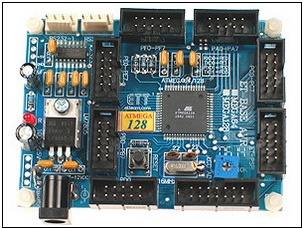
\includegraphics[scale=0.35]{./image/PESTA/kit/DevBoard_2.jpg}
	\end{figure}
	O projeto consiste em fazer uma balança tendo como supporte os equipamentos mencionados.\\
	Como demostrado na capa sua montagem, este tem um display para visualizar a massa dos objectos colocados no prato, o microcontrolador usado é um \textbf{Atmega 128} na qual trata o processamento de todo a informação e controlo.\\
	Botões de controlo para \textit{offset} e calibração do \textit{Gain Factor} também \textit{leds} para indicar o \textit{status} são integrados neste trabalho, é um interface intuitivo.
\end{frame}
%%%%%%%%%%%%%%%%%%%%%%%%%%%%%%%%%%%%%%%%%%%%%%%%%%%%%%%%%%%%%%%%
